\documentclass{article}
\usepackage{graphicx}
\usepackage{float}
\usepackage{booktabs}
\usepackage{amsmath}
\usepackage{amssymb}
\usepackage{iclr2026_conference,times}

\input{math_commands.tex}

\usepackage{hyperref}
\usepackage{url}
\usepackage{subcaption}

\graphicspath{{figs/}}

% Tighten figure spacing.
\setlength{\textfloatsep}{6pt plus 1pt minus 1pt}
\setlength{\floatsep}{6pt plus 1pt minus 1pt}
\setlength{\intextsep}{6pt plus 1pt minus 1pt}
\setlength{\abovecaptionskip}{2pt}
\setlength{\belowcaptionskip}{0pt}

\title{A Heterogeneous Relational ST-GNN for NBA Trajectory Prediction}

\author{
Name 1 \\
\texttt{email1}
\AND
Name 2 \\
\texttt{email2}
\AND
Julien Stalhandske \\
\texttt{julien.stalhandske@epfl.ch}
\AND
Missipsa M'Hamed Annane \\
\texttt{missipsa.annane@epfl.ch}
}

\iclrfinalcopy
\begin{document}
\maketitle

\begin{abstract}
We predict the next $H{=}12$ frames of an NBA play given a $C{=}8$-frame context
of the $(x, y)$ positions of $10$ players and the ball. The $11$ entities of
three distinct types interact through physically meaningful relations
(teammate, opponent, possession), so the problem is a natural fit for a
heterogeneous graph neural network. We build a per-timestep relational graph
with five learned relation types, push it through a stack of
\textit{HeteroSTGCN} cells (RGAT $\rightarrow$ GRU $\rightarrow$ LayerNorm),
and roll the predicted positions back into the input autoregressively. A
court-symmetric data augmentation -- axis flips, team-label swap, within-team
player permutation -- multiplies the effective training set by
$\sim\!10^5$ because the architecture is equivariant under all four
transformations. Averaged over five seeds, the model attains a validation MSE
of $3.25\pm 0.16$~ft\textsuperscript{2}; the per-horizon ADE grows almost
linearly to $3.49$~ft at step~$12$, with the ball contributing $2.6\times$
the ADE of either team.
\end{abstract}

\section{Introduction}
\label{sec:intro}

Predicting the short-horizon motion of all entities on a basketball court is
challenging because the interactions between players and the ball are
heterogeneous. The EPFL EE-452 Kaggle task formalises this as a
sequence-to-sequence problem: given the $11$ entity positions over
$C{=}8$ context frames, predict the next $H{=}12$ frames.

Two properties of the task drive our modelling choices. First, the
$N{=}11$ entities are not exchangeable: three node types (Team\_A, Team\_B,
Ball) and the relation between two entities depends on \emph{which} two they
are -- a heterogeneous graph with multiple relation types is the natural
backbone. Second, the court is symmetric about both axes, team labels are
arbitrary, and the five players on a team are interchangeable. Any
equivariant model can therefore be trained on an effective dataset
$2^3{\cdot}(5!)^2{=}115{,}200$ times larger than the raw files, which we
exploit with on-the-fly augmentation.

Our main empirical findings are: (a)~train and validation losses overlap inside
their $95\%$ confidence bands across five seeds, so the architecture is not
overfit at $50$~epochs; (b)~error grows almost linearly with prediction
horizon -- the expected signature of autoregressive rollout error
accumulation; and (c)~the ball dominates the error budget at $2.6\times$ the
ADE of either team, suggesting a ball-specific specialisation is the
highest-leverage follow-up.

\section{Method}
\label{sec:method}

\subsection{Dataset and Task}

The training set contains $4{,}968$ sequences of length $T\!\in\![20, 225]$
(median $30$); the test set has $1{,}243$ files of exactly $8$ frames. At each
frame the eleven entities are stored as
$(x, y, \mathrm{entity\_id}, \mathrm{team\_id})$ with
$\mathrm{team\_id}{\in}\{-1, 0, +1\}$ marking Team\_A, the Ball, and Team\_B.
The spread of sequence lengths yields $189{,}370$ usable
$(C{+}H)$-windows, $38$ per sequence on average -- enough that the model is
not data-starved. Figure~\ref{fig:dataset} shows the basic dataset
descriptors. The court-occupancy heatmap is mirror-symmetric about both
axes for the two teams and the ball concentrates sharply at the two baskets
at $x\!\approx\!\pm 43$~ft, empirical confirmation that the symmetries we
want to encode are present in the data. Possession (closest player to ball)
is balanced to $49.5\%\,/\,50.5\%$ across $283{,}762$ frames.

\begin{figure}[H]
  \centering
  \begin{subfigure}[t]{0.33\textwidth}
    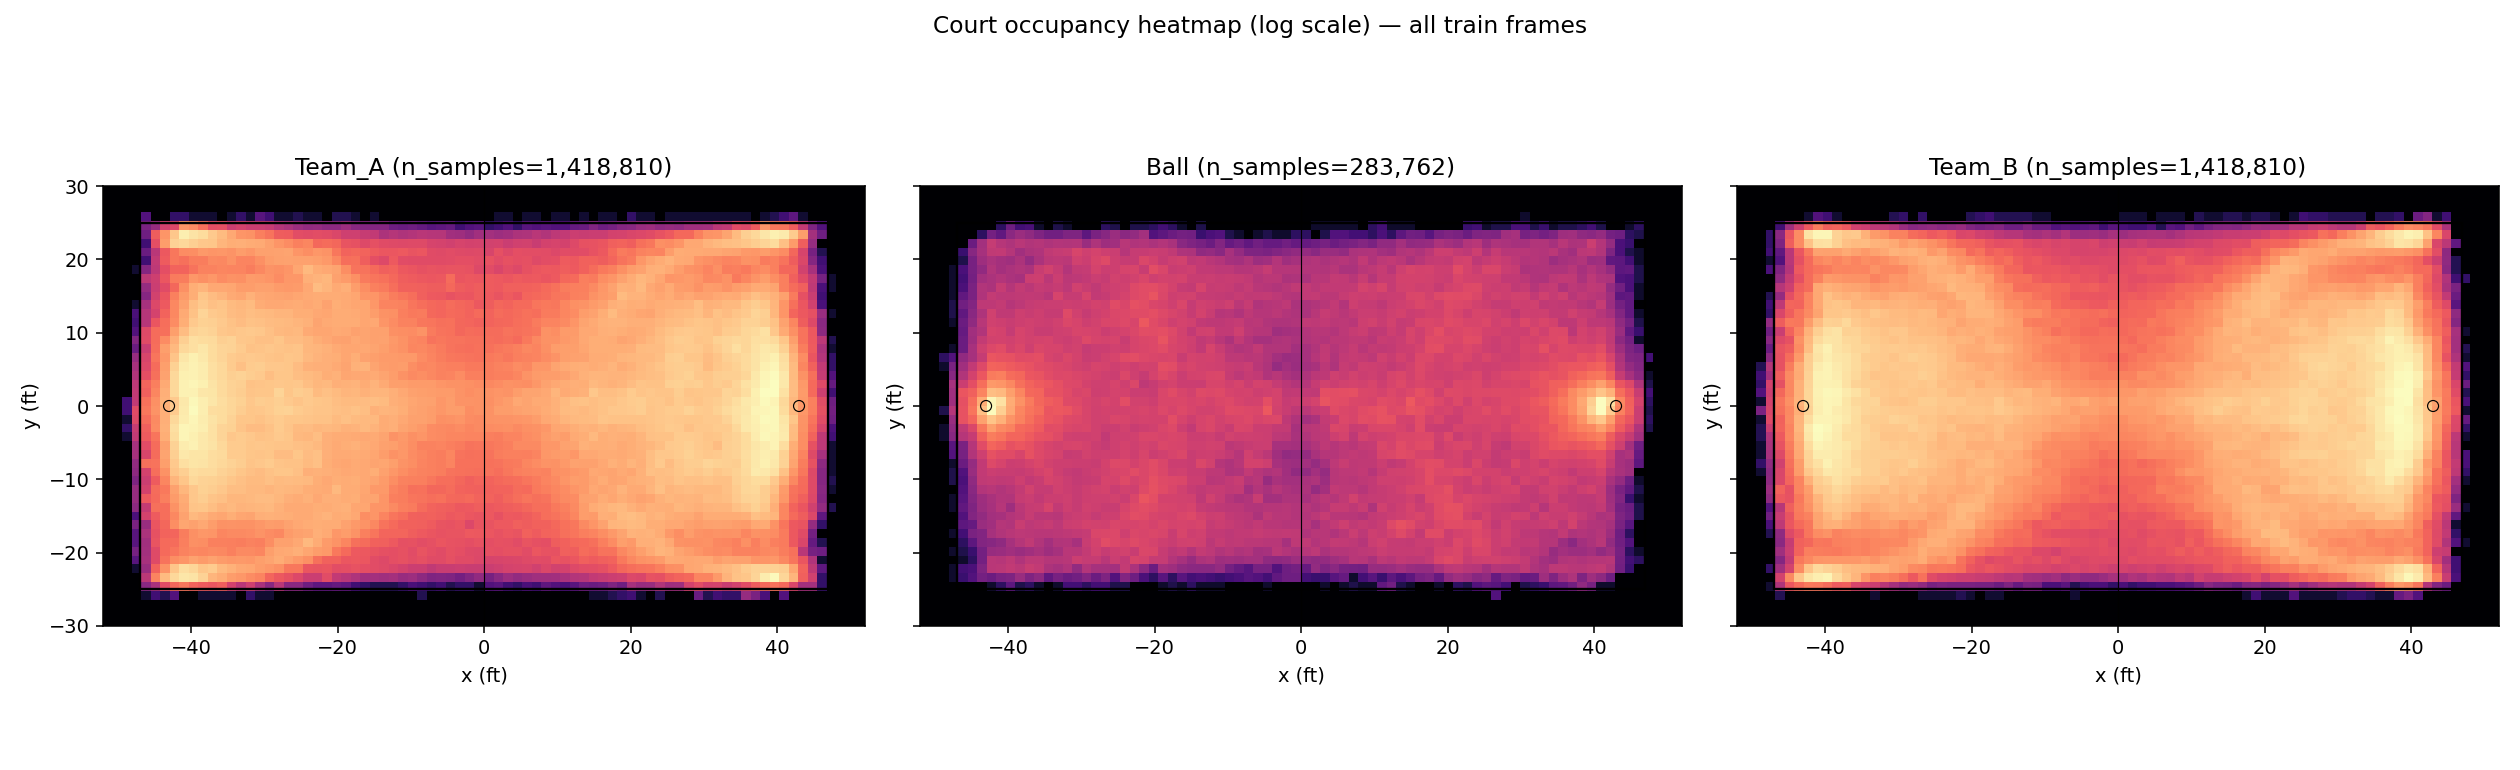
\includegraphics[width=\linewidth]{court_heatmap.png}
    \caption{Court occupancy (log).}
  \end{subfigure}\hfill
  \begin{subfigure}[t]{0.33\textwidth}
    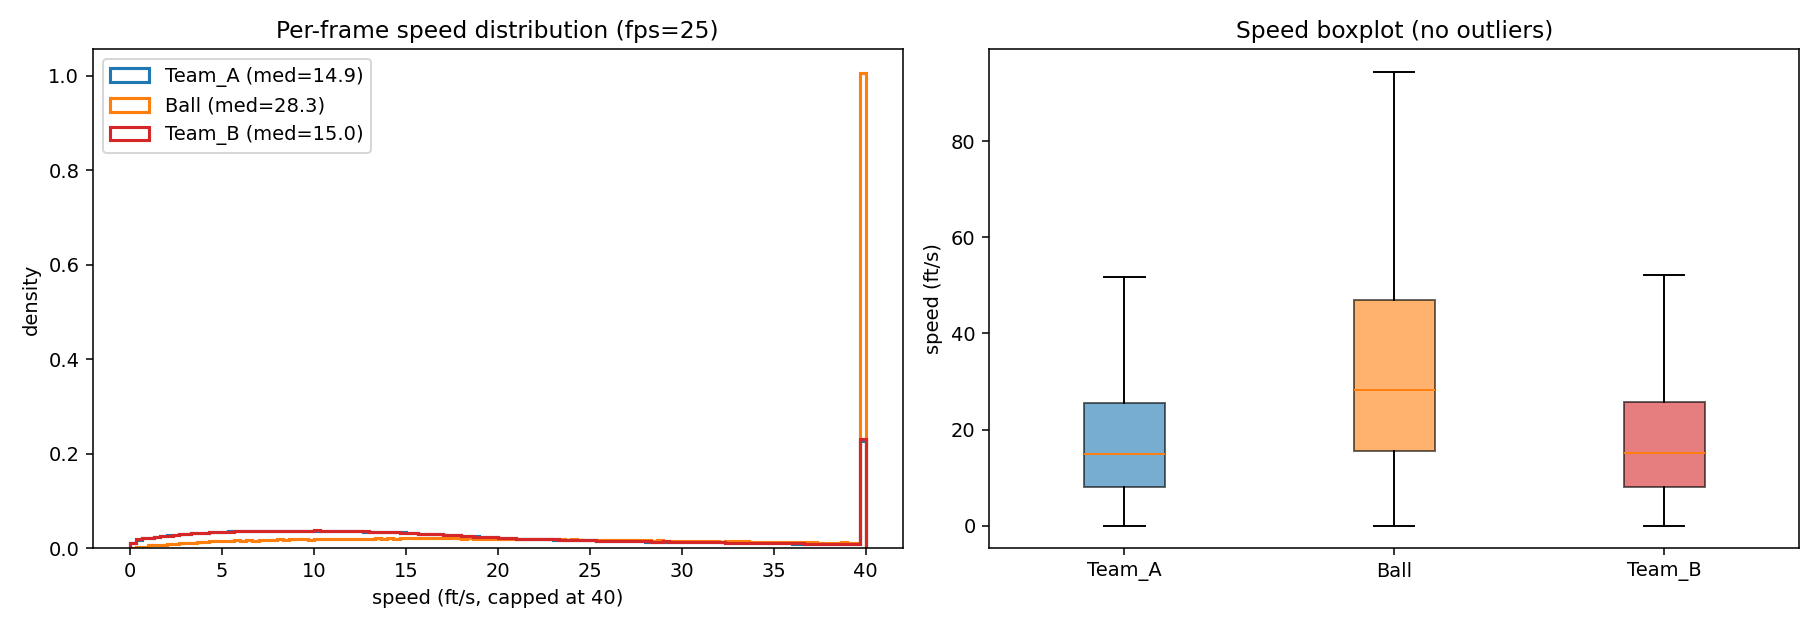
\includegraphics[width=\linewidth]{speed_distribution.png}
    \caption{Speed by entity type.}
  \end{subfigure}\hfill
  \begin{subfigure}[t]{0.32\textwidth}
    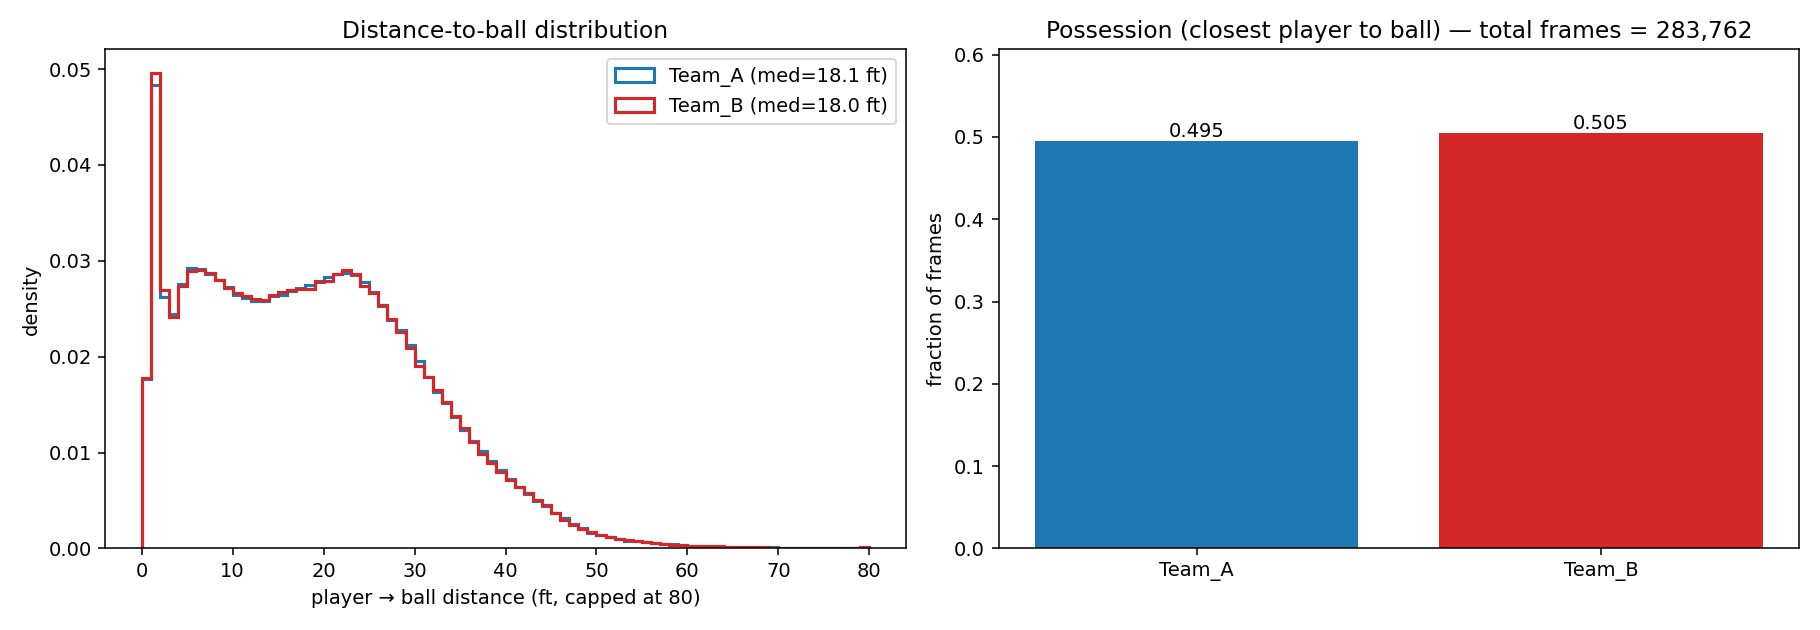
\includegraphics[width=\linewidth]{distance_to_ball.png}
    \caption{Player--ball distance.}
  \end{subfigure}
  \caption{Train-set diagnostics. Occupancy is mirror-symmetric, the ball
  moves about twice as fast as the players ($28.3$ vs.\ $15.0$~ft/s median),
  and the player--ball distance has a sharp ball-handler mode at $\sim\!2$~ft.}
  \label{fig:dataset}
\end{figure}

\subsection{Heterogeneous Graph}

Each batch sample induces a complete directed graph on $N{=}11$ nodes with
$N^2{=}121$ edges, but each edge carries one of five \emph{relation types}
determined by the static team labels at $t{=}0$: $\{0{:}\text{teammate},
1{:}\text{opponent}, 2{:}\text{player}{\to}\text{ball}, 3{:}\text{ball}
{\to}\text{player}, 4{:}\text{self-loop}\}$. This yields
$40\!+\!50\!+\!10\!+\!10\!+\!11$ edges per sample
(Figure~\ref{fig:graph}, right). The relation matrix encodes node-type
partitioning explicitly and is the only piece of structural information the
network needs at construction time. Edges are rebuilt once per batch (since
relations are static in time) while per-edge geometric features
$[\Delta x, \Delta y, \lVert\Delta\rVert]$ are recomputed every step from the
rolled-out positions.

\begin{figure}[H]
  \centering
  \begin{subfigure}[t]{0.52\textwidth}
    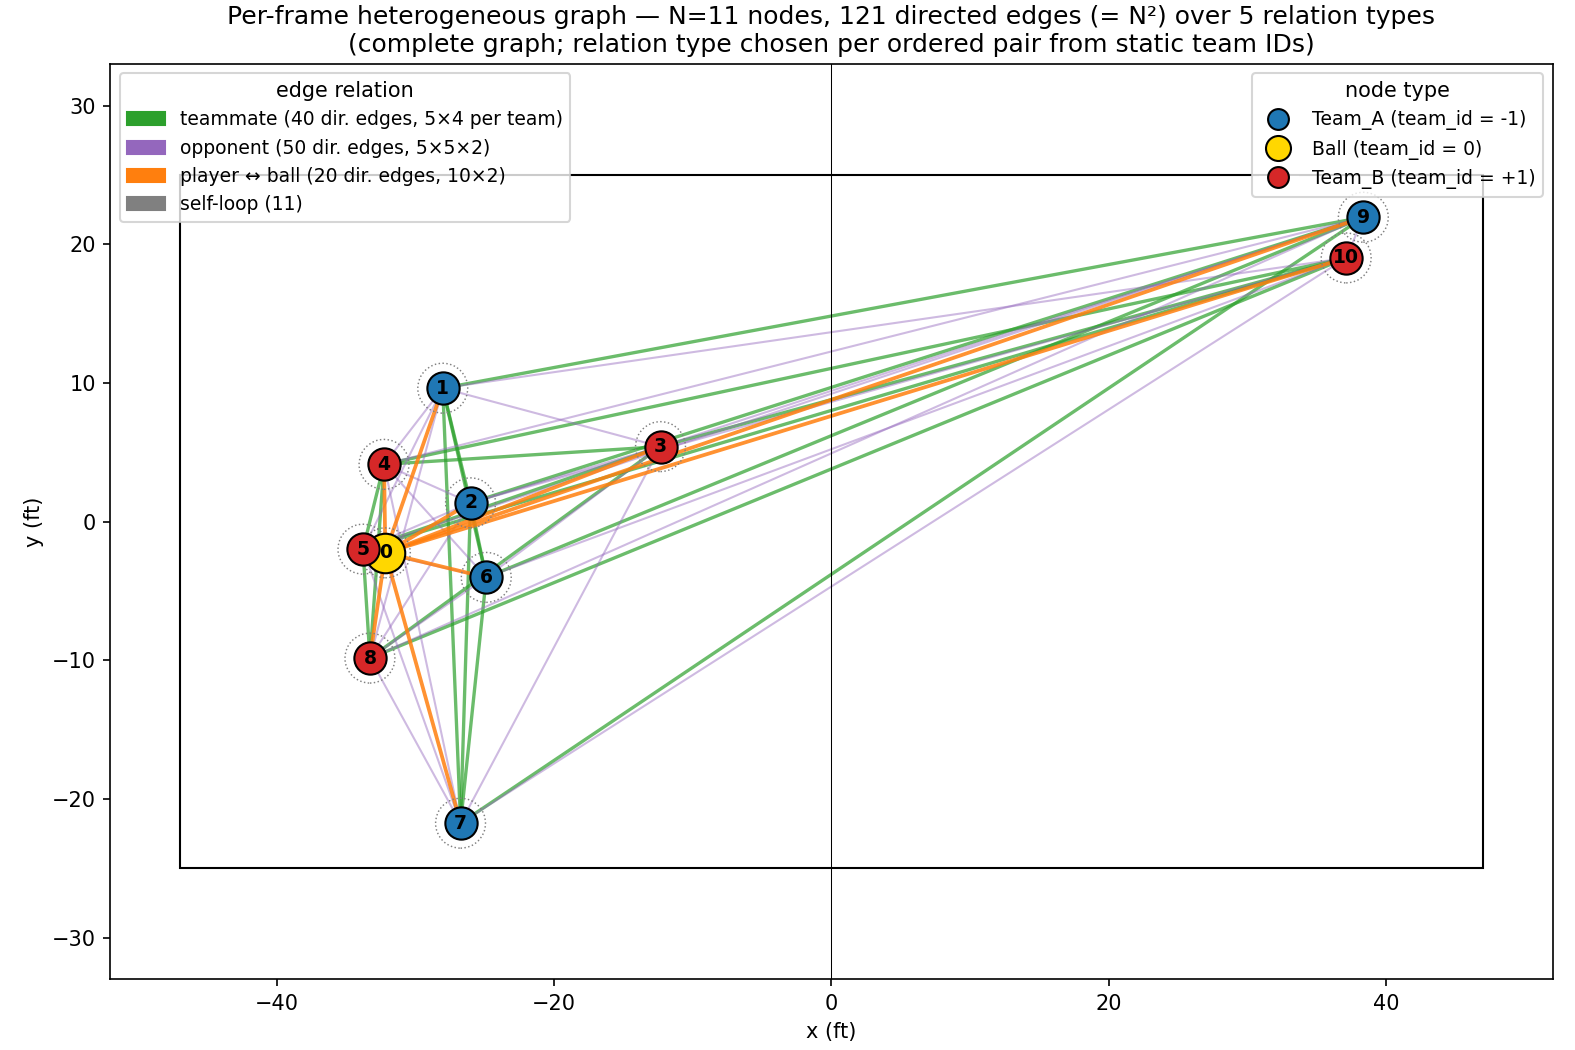
\includegraphics[width=\linewidth]{hetero_graph.png}
  \end{subfigure}\hfill
  \begin{subfigure}[t]{0.46\textwidth}
    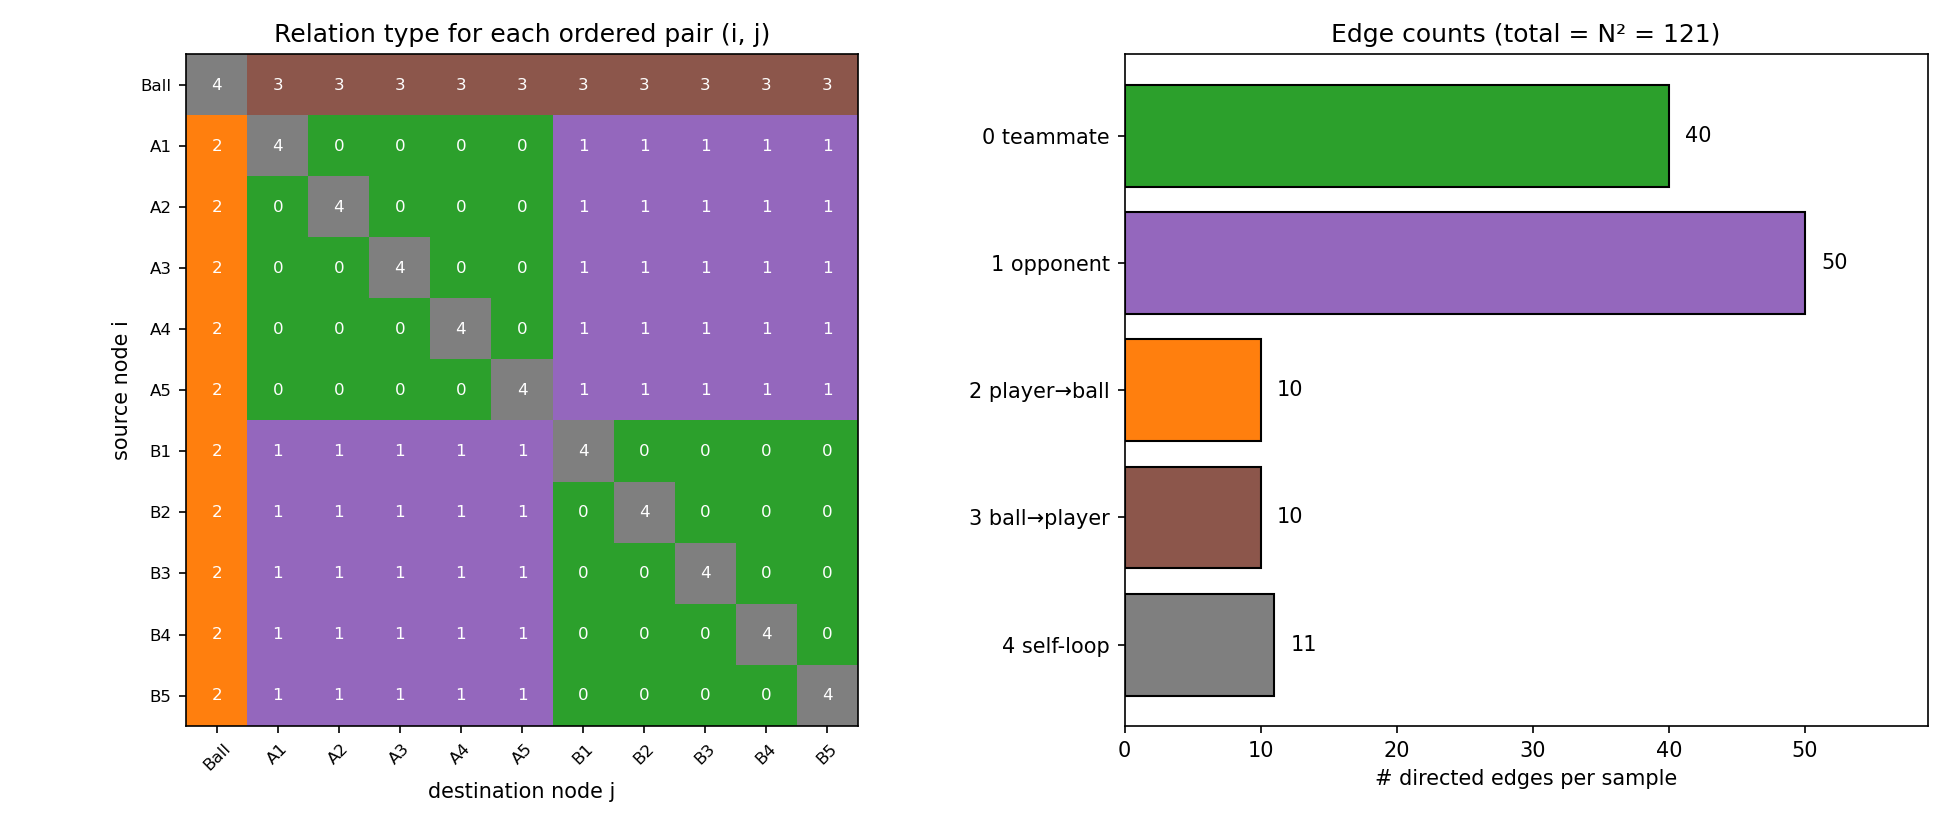
\includegraphics[width=\linewidth]{edge_type_legend.png}
  \end{subfigure}
  \caption{Heterogeneous graph construction. \textit{Left}: the five relation
  types drawn on a real frame. \textit{Right}: the relation type chosen for
  each ordered pair $(i, j)$ and the per-relation edge count.}
  \label{fig:graph}
\end{figure}

\subsection{Model Architecture}

The backbone is a spatial-temporal heterogeneous graph RNN. At each of the
$T{=}20$ timesteps the model builds a per-node feature vector
(Figure~\ref{fig:model}c) consisting of the current position, finite-difference
velocity, kinematics (acceleration, speed, heading
$(\cos\theta,\sin\theta)$), the static $(\mathrm{entity\_id},
\mathrm{team\_id})$ fields, and a possession signal $(d_\text{ball},
\mathrm{softmax}(-d/\tau))$ with $\tau{=}5$~ft (Figure~\ref{fig:model}d). The
softmin assigns a peaked probability to the ball-handler and is masked to
zero at the ball itself.

The features feed a stack of \textbf{HeteroSTGCN} cells
(Figure~\ref{fig:model}b); each cell is an RGAT convolution
\citep{busbridge2019rgat} (with the five relation types and per-edge geometric
features as edge attributes) followed by \texttt{ReLU}, a \texttt{GRUCell}
\citep{cho2014gru} that keeps a per-layer hidden state across all twenty
timesteps, and \texttt{LayerNorm}. From layer $\ell{\ge}1$ the input to the
next cell adds a residual, so the receptive field on the heterogeneous graph
grows by one hop per layer without erasing earlier features. A two-layer MLP
projects the final hidden state to a $2$-D coordinate delta $\Delta_{xy}$ and
the rollout proceeds via $p_{t+1}{=}p_t+\Delta_{xy}$. During the context
window the input position is ground truth; during the horizon it is the
model's own previous prediction (Figure~\ref{fig:model}a).

\begin{figure}[H]
  \centering
  \begin{subfigure}[t]{0.49\textwidth}
    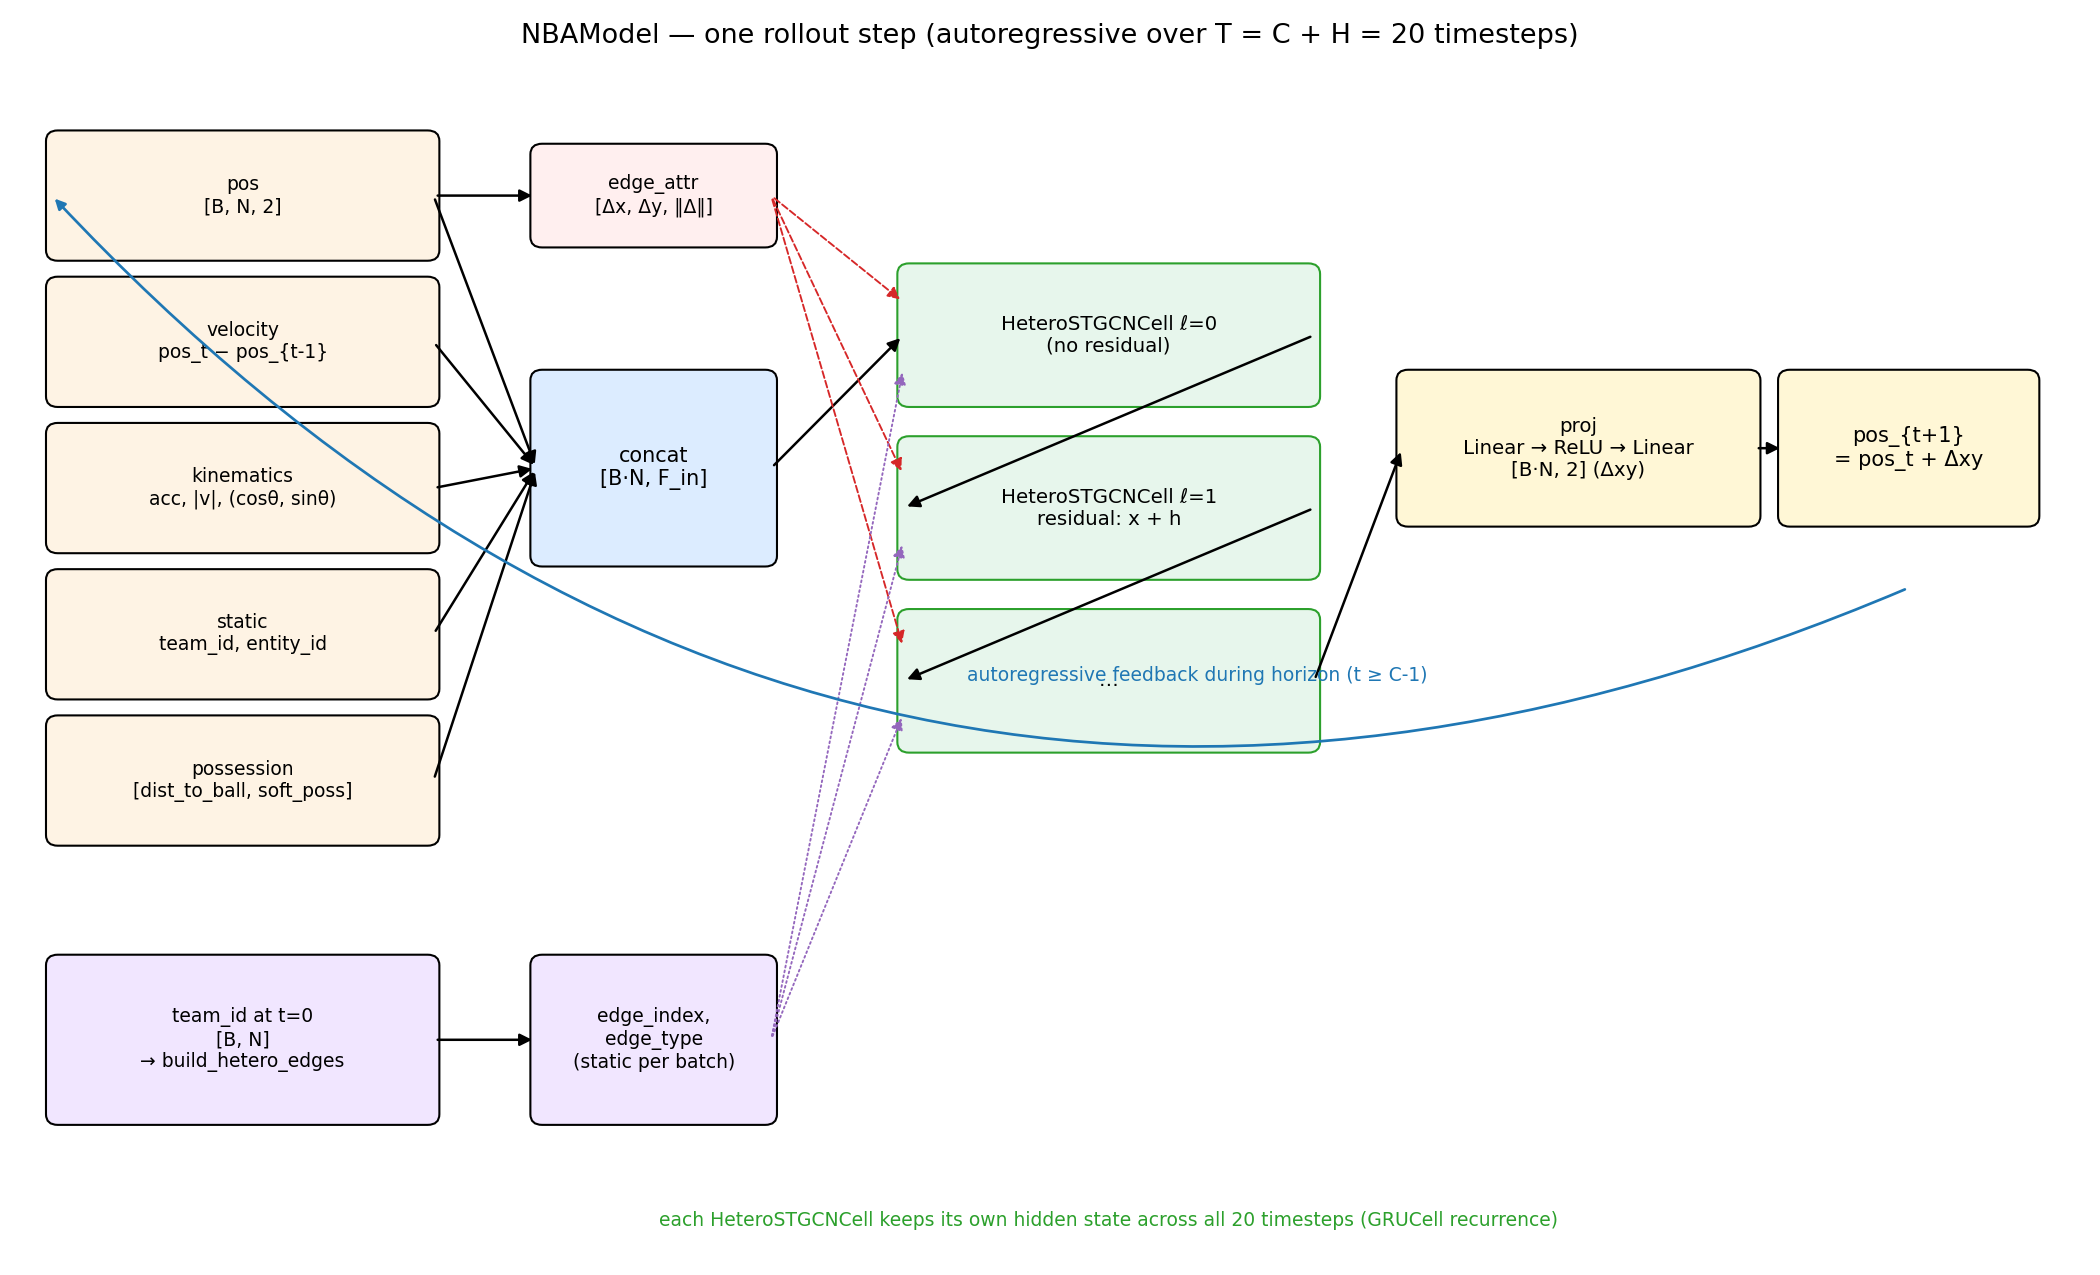
\includegraphics[width=\linewidth]{architecture.png}
    \caption{One rollout step.}
  \end{subfigure}\hfill
  \begin{subfigure}[t]{0.49\textwidth}
    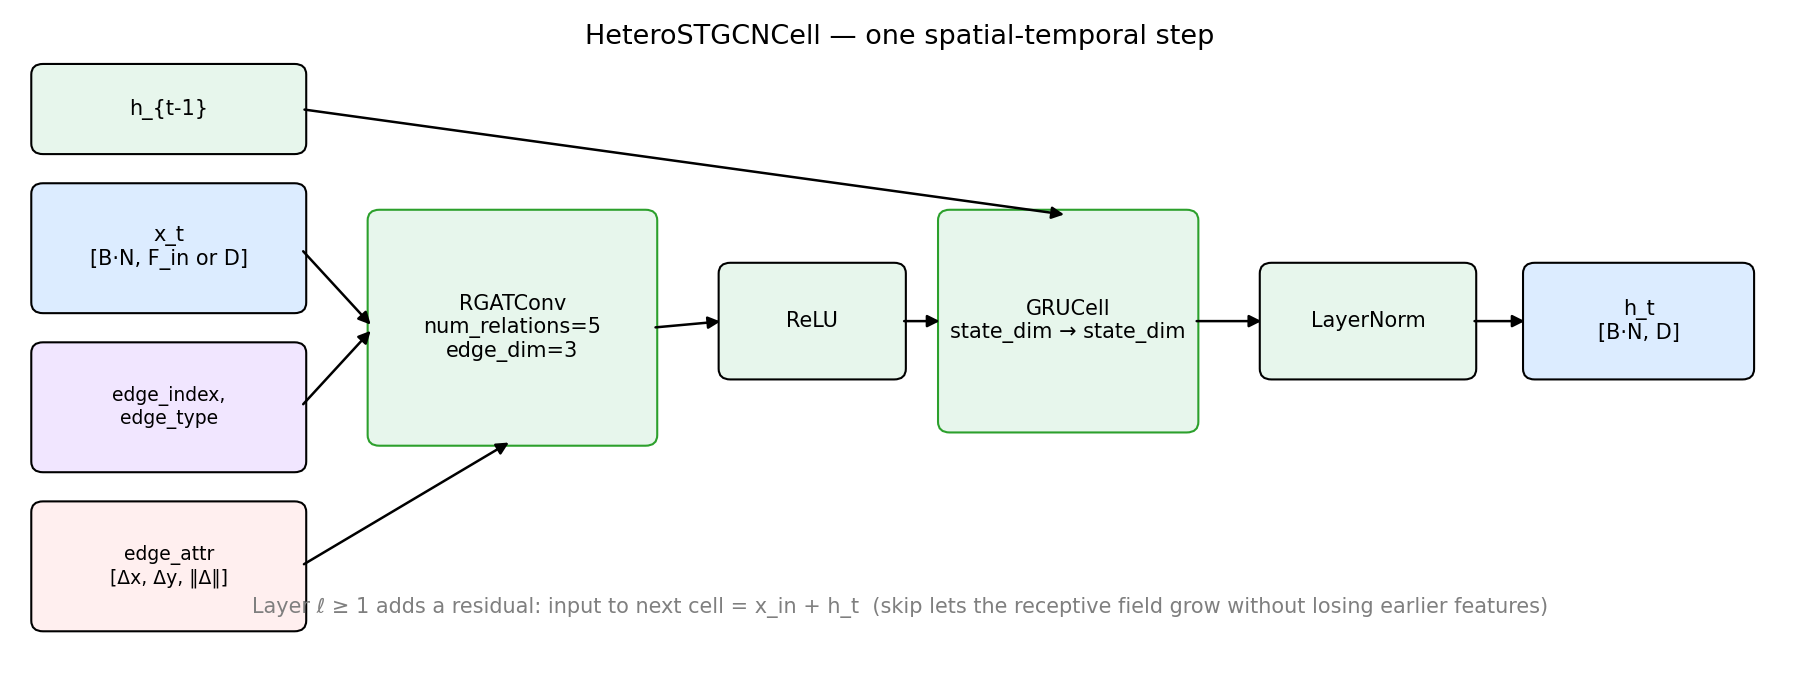
\includegraphics[width=\linewidth]{stgcn_cell.png}
    \caption{HeteroSTGCN cell internals.}
  \end{subfigure}\\[2pt]
  \begin{subfigure}[t]{0.55\textwidth}
    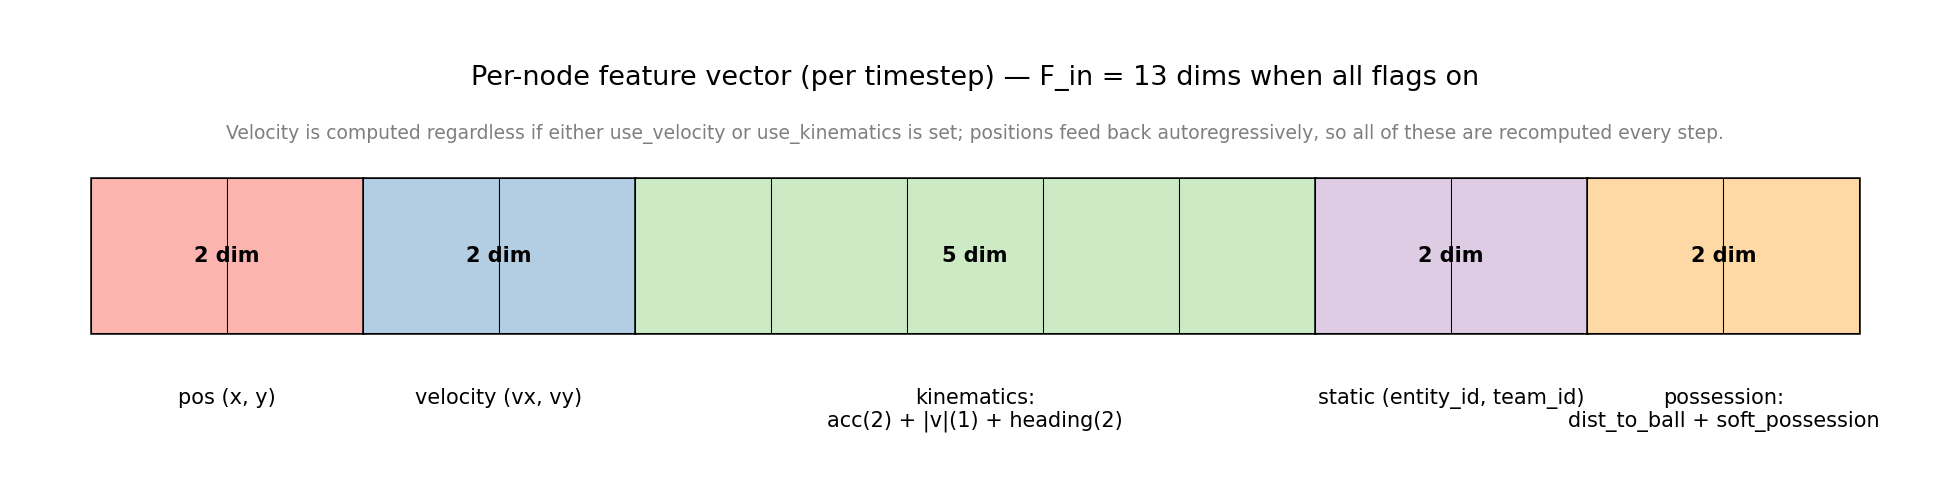
\includegraphics[width=\linewidth]{feature_stack.png}
    \caption{Per-node feature vector ($F_\text{in}{=}13$ with all flags on).}
  \end{subfigure}\hfill
  \begin{subfigure}[t]{0.43\textwidth}
    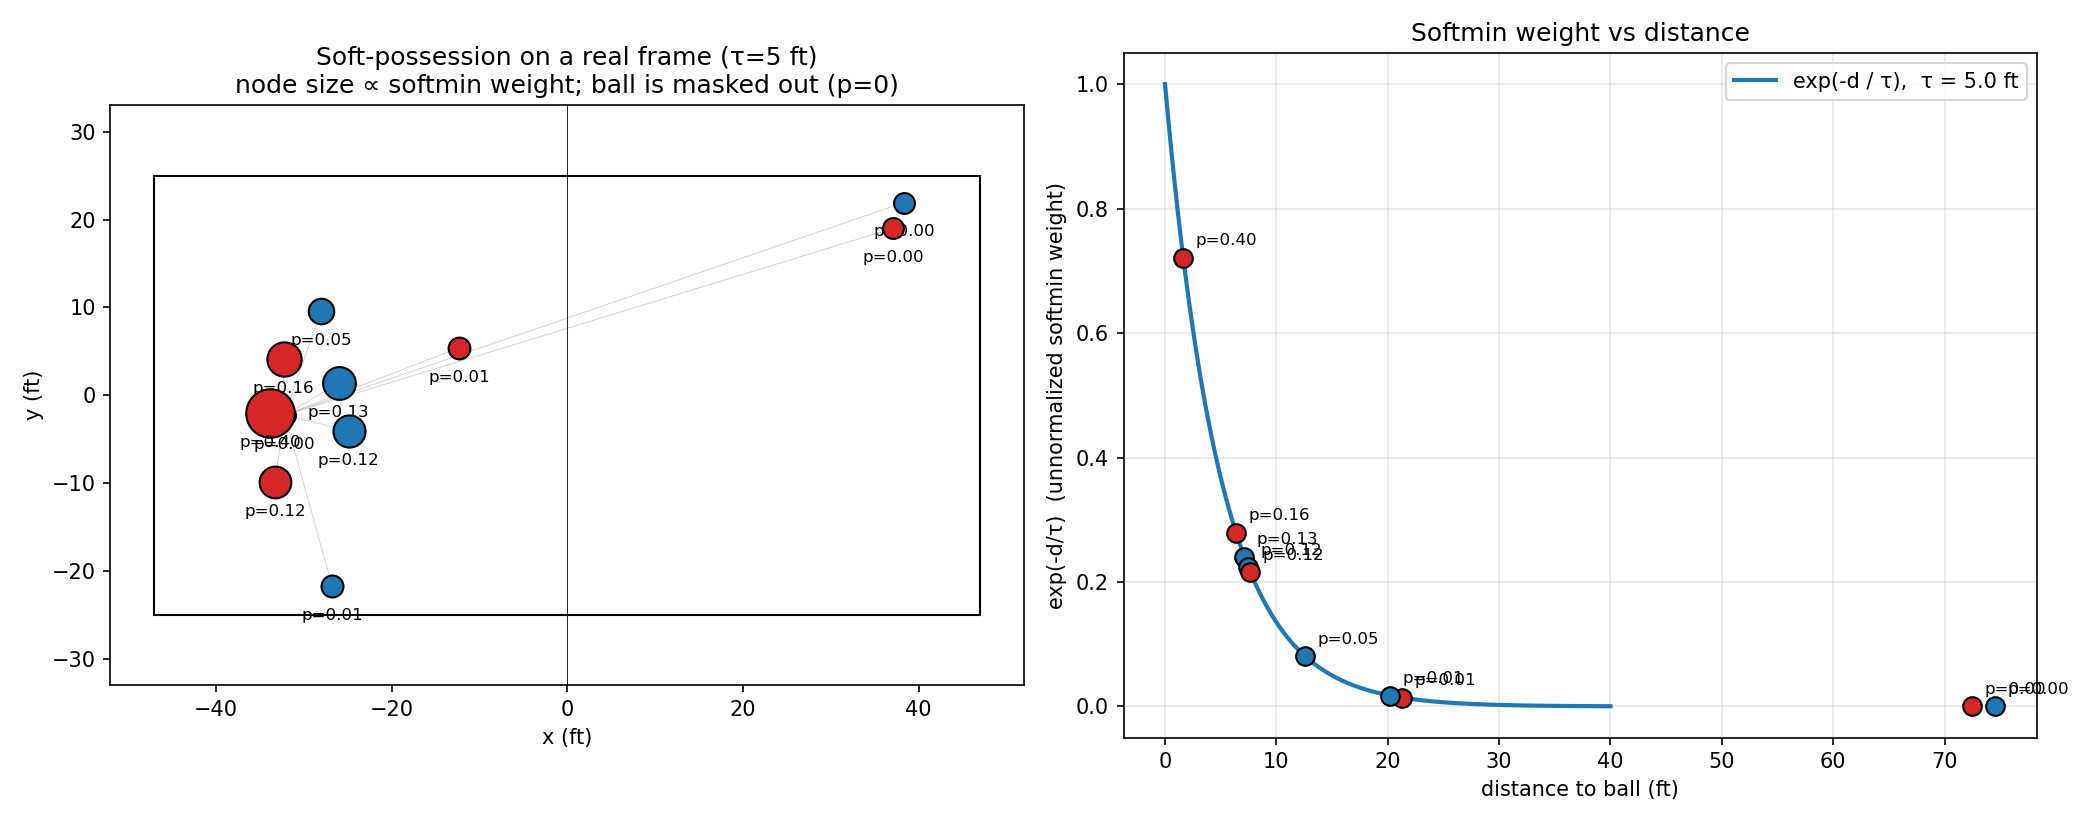
\includegraphics[width=\linewidth]{possession_softmin.png}
    \caption{Soft-possession ($\tau{=}5$~ft).}
  \end{subfigure}
  \caption{Model overview. The graph and the cells are shared across all
  $T{=}20$ timesteps; only the per-step inputs change between context and
  horizon.}
  \label{fig:model}
\end{figure}

\subsection{Training}

We minimise MSE over the full $[H, B{\cdot}N, 2]$ prediction tensor with Adam
($\eta{=}10^{-3}$, weight decay $5{\times}10^{-4}$) and
\texttt{CosineAnnealingLR} ($\eta_\text{min}{=}10^{-5}$,
$T_\text{max}{=}\text{epochs}$). Gradients are clipped at
$\lVert\cdot\rVert_2{=}10$. The model interior runs in normalized units, but
all reported metrics are in feet.

A central design decision is the on-the-fly augmentation: every fetched
$(C,H)$ window is independently x-flipped, y-flipped, team-swapped, and
within-team permuted with probability $1/2$ each. The court is symmetric
about both axes, and the heterogeneous edge construction depends only on
team-\emph{equality} (not on which team is $+1$ vs.\ $-1$), so all four
transformations preserve the graph topology and the loss -- they are true
symmetries of the model.

\section{Results}
\label{sec:results}

\paragraph{Experimental setup.} The best configuration uses $C{=}8$, $H{=}12$,
$\mathrm{state\_dim}{=}128$, a single \textsc{HeteroSTGCN} layer, batch
size~$64$, five $(\text{seq\_idx}, \text{start})$ windows per training
sequence per epoch, and $50$~epochs with augmentation. We train five
independent models, varying only the master seed (which controls weight
initialisation, train/val split, sampler shuffling, and CUDA RNG). All
numbers below are mean $\pm$ $95\%$ Student-$t$ confidence interval over the
five seeds.

\begin{figure}[H]
  \centering
  \begin{subfigure}[t]{0.49\textwidth}
    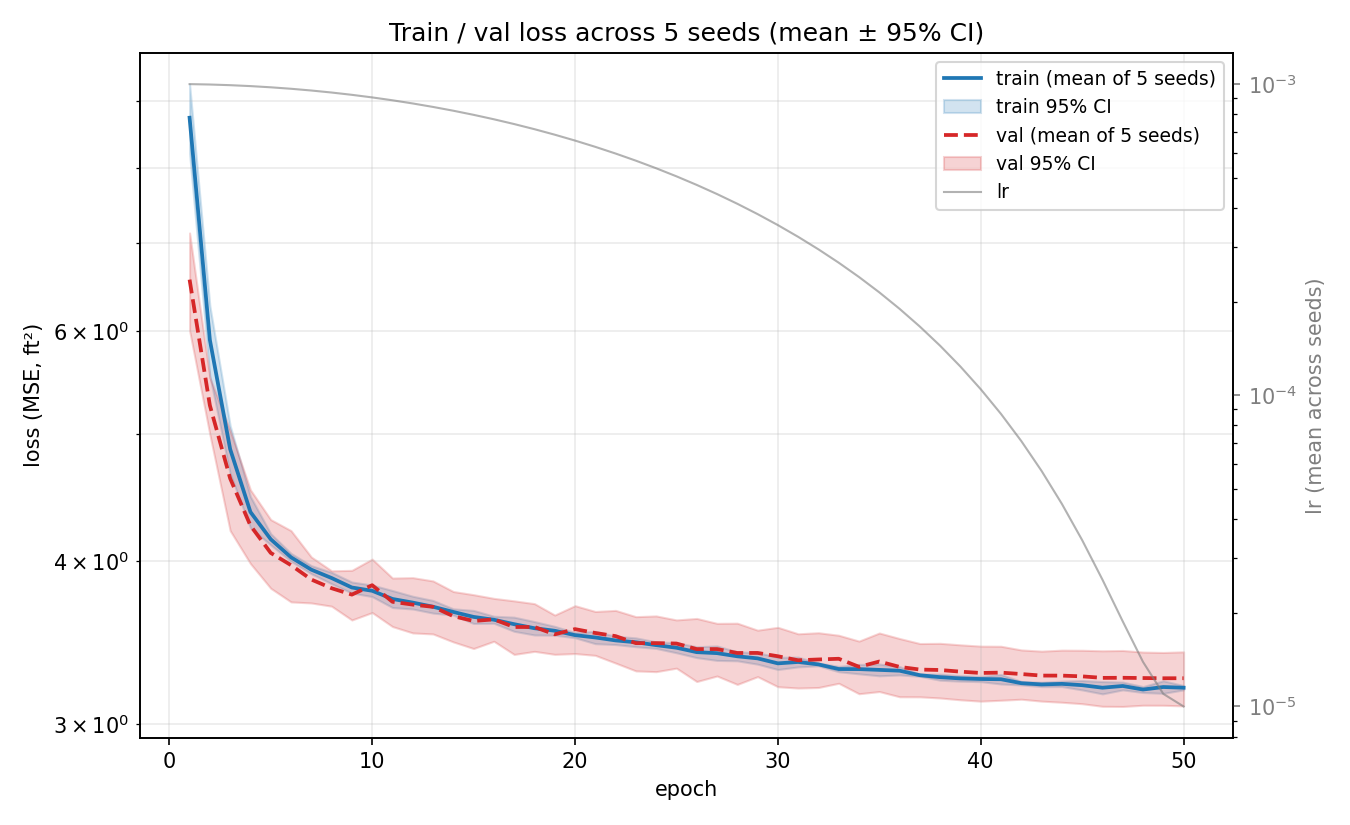
\includegraphics[width=\linewidth]{loss_curves_seeds.png}
    \caption{Train/val loss across 5 seeds.}
  \end{subfigure}\hfill
  \begin{subfigure}[t]{0.49\textwidth}
    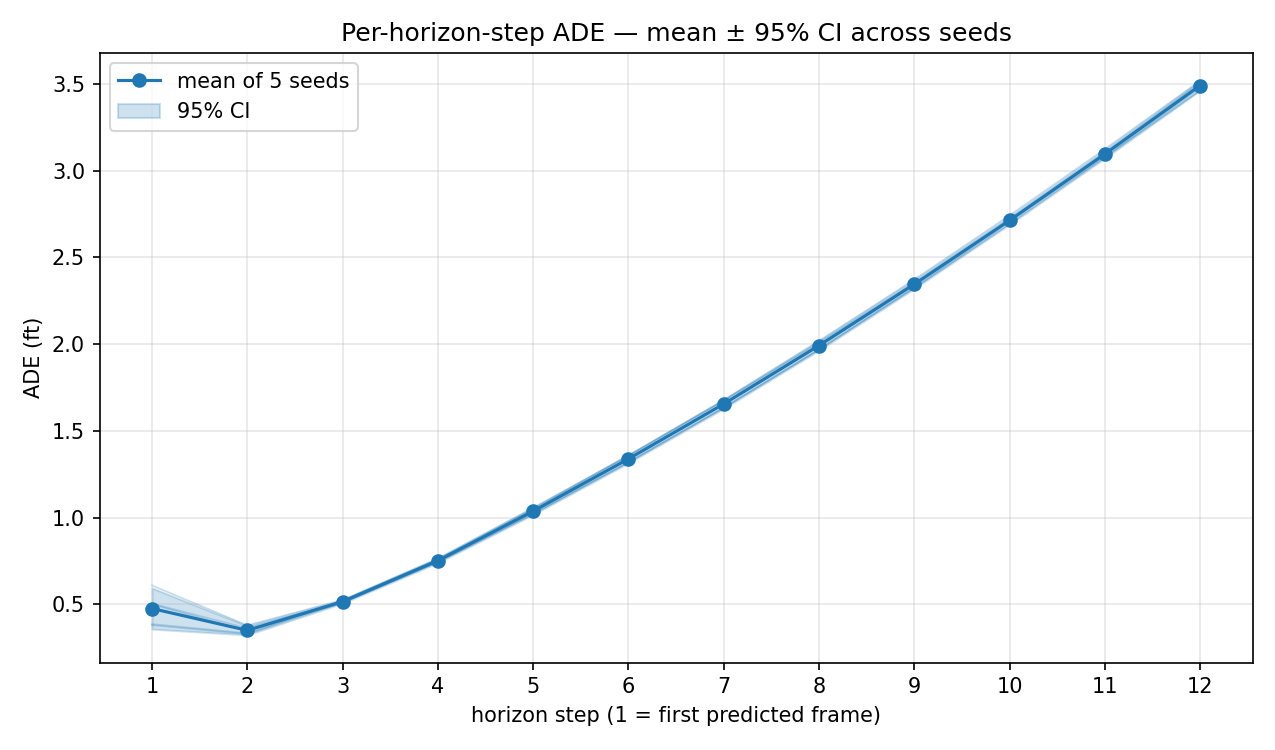
\includegraphics[width=\linewidth]{per_horizon_ade_seeds.png}
    \caption{Per-horizon-step validation ADE.}
  \end{subfigure}\\[2pt]
  \begin{subfigure}[t]{0.49\textwidth}
    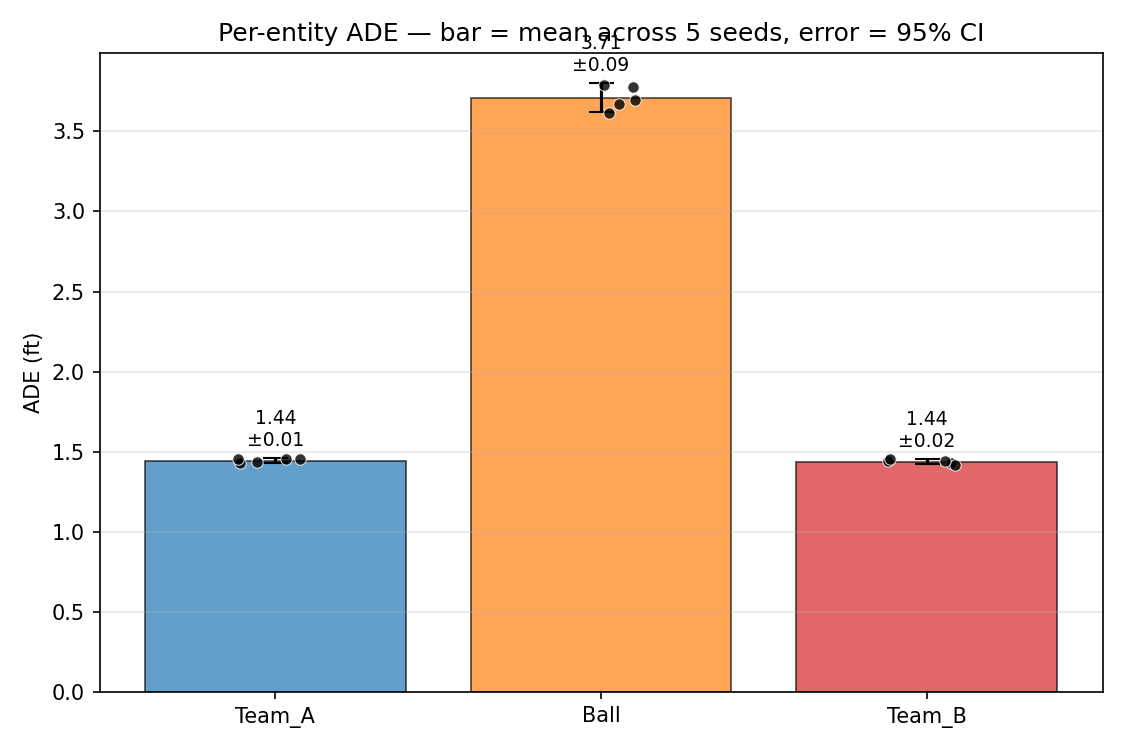
\includegraphics[width=\linewidth]{per_entity_ade_seeds.png}
    \caption{Per-entity validation ADE.}
  \end{subfigure}\hfill
  \begin{subfigure}[t]{0.49\textwidth}
    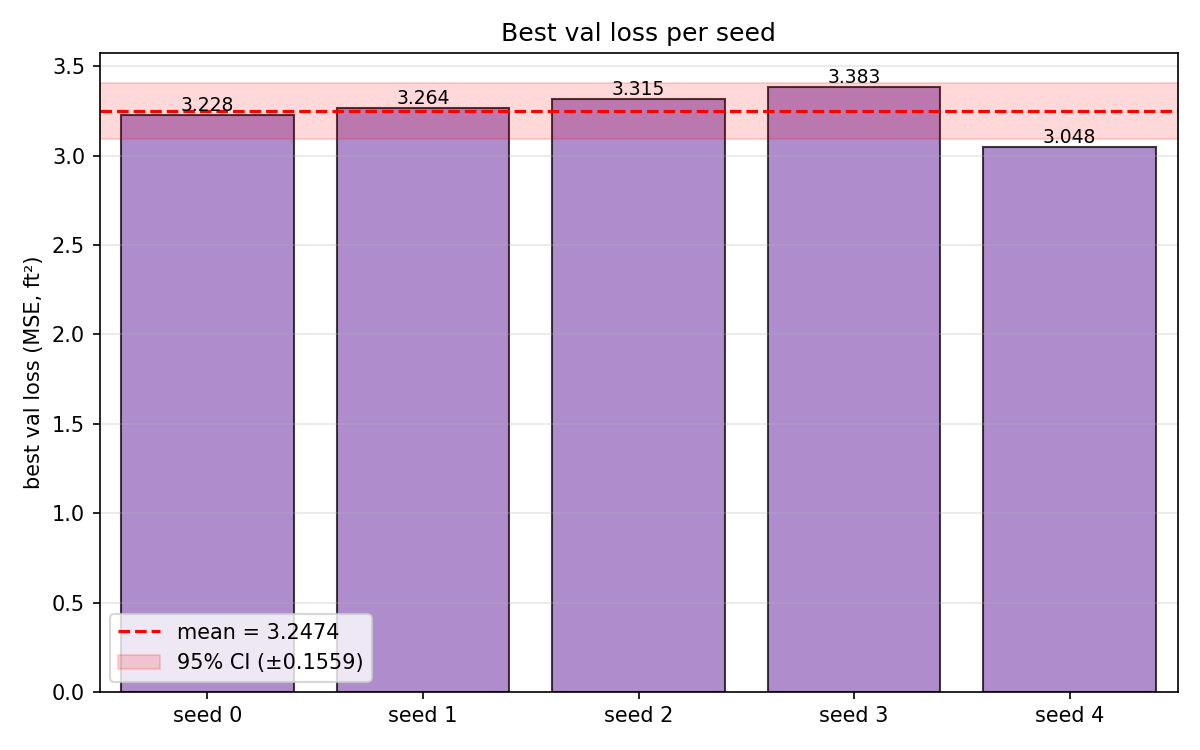
\includegraphics[width=\linewidth]{best_val_loss_seeds.png}
    \caption{Best val loss per seed.}
  \end{subfigure}
  \caption{Multi-seed aggregate results ($n{=}5$, $95\%$ CI). Bands and error
  bars are tight on every metric except step-$1$ ADE, where seeds disagree
  more.}
  \label{fig:seeds}
\end{figure}

\paragraph{Training stability.} Final-epoch training loss is
$3.20\pm 0.01$ and validation $3.25\pm 0.16$~ft\textsuperscript{2}; the
best-checkpoint validation loss is $3.25$~ft\textsuperscript{2} (range
$[3.05, 3.38]$). Train and validation curves overlap inside their bands
throughout training (Figure~\ref{fig:seeds}a), so the model is not over-fit
at $50$~epochs even without explicit early stopping.

\paragraph{Horizon scaling.} Per-horizon ADE grows almost linearly from
$0.35$~ft at step~$2$ to $3.49$~ft at step~$12$ (Figure~\ref{fig:seeds}b).
The slope ($\sim\!0.30$~ft/frame, $\sim\!7.5$~ft/s at the assumed $25$~fps
tracking rate) is roughly half the median player speed. This is the
expected signature of autoregressive rollout: when the input at step $t{+}1$
is the model's own output at step $t$, small per-step errors accumulate.

\paragraph{Symmetry between teams.} Per-entity ADE
(Figure~\ref{fig:seeds}c) reads $1.44\pm 0.01$~ft for Team\_A,
$1.44\pm 0.02$~ft for Team\_B, and $3.71\pm 0.09$~ft for the Ball. The two
team errors agree to within $0.01$~ft -- direct empirical evidence that the
augmentation makes the learned model team-equivariant in practice.

\paragraph{The ball dominates the error budget.} Although there is only one
ball against ten players, its ADE is $2.6\times$ that of either team -- the
unweighted MSE loss therefore puts only $1/11$th of its mass on the ball even
though the ball drives most of the residual error.

\section{Conclusion}
\label{sec:conc}

A relational graph attention backbone wrapped in a GRU recurrence is a
strong, low-variance baseline for short-horizon NBA trajectory prediction,
reaching $3.25\pm 0.16$~ft\textsuperscript{2} validation MSE across five
seeds with no early stopping. The five relation types let one set of
parameters serve very different physical interactions, and the
court-symmetric augmentation -- valid only because relations depend on
team-\emph{equality} -- multiplies the effective dataset by $\sim\!10^5$;
the two-decimal-place agreement between Team\_A and Team\_B ADEs across
five seeds confirms equivariance in practice. The remaining gap is the
ball-vs-player asymmetry: a ball-weighted loss or an entity-specific output
head (already supported by \texttt{use\_ball\_head}) are the most promising
follow-ups.

\section*{Statement of Contributions}
\textbf{We hereby state that all the work presented in this report is that of the authors.}

\bibliography{references}
\bibliographystyle{iclr2026_conference}

\end{document}
